\documentclass[12pt,a4paper]{article}
\usepackage[top=2.7cm, bottom=2cm, left=2cm, right=2cm]{geometry}
\usepackage[utf8]{inputenc}
\usepackage{CJKutf8}
\usepackage{enumitem}
\usepackage{verbatim}


%% Useful packages
\usepackage{amsmath,amssymb}
% \usepackage{subfigure}
\usepackage{graphicx,wrapfig}
\usepackage[dvipsnames,table]{xcolor}
\usepackage[table]{xcolor}
\usepackage{url}
\usepackage{setspace}
\usepackage[colorlinks=true,anchorcolor=black,linkcolor=Blue,urlcolor=RoyalBlue]{hyperref}
\usepackage[linesnumbered,ruled,vlined]{algorithm2e}
\usepackage{threeparttable}

\usepackage{tikz}
\usepackage{blindtext}
\usepackage{titlesec}
\usepackage{courier}
\usepackage{pdfpages}

\usepackage{lastpage}
\usepackage{fancyhdr}
\setlength{\headheight}{0pt}
\renewcommand{\headrulewidth}{1pt} % remove lines
\renewcommand{\footrulewidth}{0pt}
\pagestyle{fancyplain}
\fancyhf{}
\lhead{
  \textcolor{Gray}{Group 2}
}
\rhead{
  \begin{CJK}{UTF8}{bkai}
  \textcolor{Gray}{實驗結報}
  \end{CJK}
}
\lfoot{
   \textcolor{Gray}{April 1}
  }
\rfoot{
  \thepage/\pageref{LastPage}
  }

\title{\vspace{-0.5cm}
       {\bf \textcolor{black}{{\LARGE 
       \begin{CJK}{UTF8}{bkai}
       實驗物理學(二)\\
       \vspace{6pt}
        實驗結報\\
       % \vspace{60pt}
       % Fundamental Python\\
       % \vspace{6pt}
       % Basic Usage of Python
       \end{CJK}
       }}
       }
       }
\author{}
\date{}

\begin{document}
\begin{CJK}{UTF8}{bkai}

\maketitle
\thispagestyle{empty}

\vspace{10cm}
\begin{center}
{\bf \LARGE \vspace{-11cm} Fundamental Python\\
\vspace{0.25cm} Fitting Data of Simple Pendulum}\\
\vspace{13cm}
{\large Group 2}\\ \vspace{12pt}
{\large \makebox[3em][s]{洪\hspace{\fill}瑜} B125090009}\\ \vspace{6pt}
{\large \makebox[3em][s]{黃巧涵}  B122030003}\\ \vspace{6pt}
{\large \makebox[3em][s]{洪懌平} B102030019}\\ \vspace{12pt}
{\large 2025/04/01}\\
\end{center}

\clearpage
%--------------------------------------------------------------

\section{摘要}
\hfill

本實驗旨在探討單擺週期與擺長之關係,並透過Chi-square擬合方法推算重力加速度g。

儘管此主題為基礎物理定律的驗證,缺乏原創性,但在實驗物理學課程中極具訓練價值,尤其有助於理解誤差處理與數據擬合的實用性與局限性。我們將週期與擺長取對數後進行線性化處理,並使用Chi-square擬合最小化加權殘差平方和,考慮每筆資料的標準差作為權重,以提升擬合的可靠性。

實驗結果顯示,最佳擬合參數為斜率$m=0.4802$、截距$b=0.7927$,對應估算之重力加速度為$g=9.969 \,m/s^2$,相對誤差約 1.66\%。卡方統計量$\chi^2=0.1525$,顯著小於自由度,推測可能為誤差估計偏大或模型過擬合所致。與其他方法(如least squares與MCMC)相比,Chi-square擬合在誤差加權上的應用雖理論合理,但若未妥善估算誤差,仍可能導致擬合結果過於樂觀。根據本次擬合結果與殘差圖分析,模型整體表現良好,無明顯系統性偏差。

\section{前言}
%p value、看要不要把預習問題改成實驗原理;實驗原理(含LS、curve_fit、MCMC、chi)

\subsection{Simple Pendulum}
\hfill

A simple pendulum is conventionally defined as a set of a massless and tough stick or wire whose length is $L$, one side rooted to a fixed point and the other attached to a point mass source $m$. (See Fig.\ref{fig:simple_pendulum})

\begin{figure}[h]
    \centering
    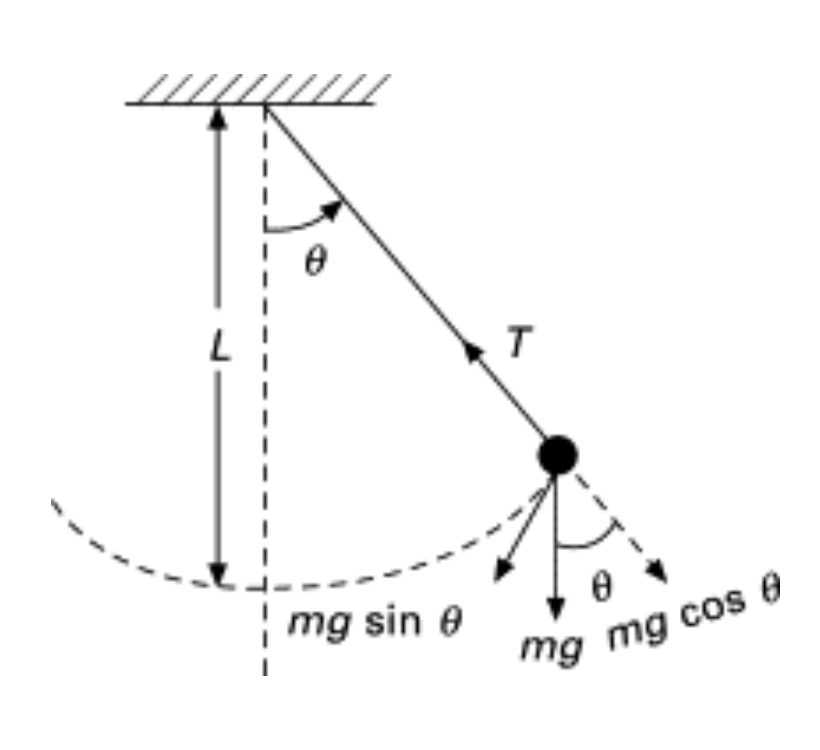
\includegraphics[width=0.5\linewidth]{simple_pendulum.png}
    \caption{Demonstration of a simple pendulum. (Credit: \href{https://www.sciencedirect.com/topics/engineering/simple-pendulum}{This site})}
    \label{fig:simple_pendulum}
\end{figure}

Using Newton's Second Law, we can get 
\begin{equation}\label{eq:pend_eq}
    mL\frac{d^2\theta}{dt^2}=-mgsin\theta
\end{equation}

As $\theta\sim0$, i.e., under the small-angle approximation, $sin\theta\sim\theta$ (if we take the first Taylor expansion), Eq. \ref{eq:pend_eq} can then be simplified to:
\begin{equation}
    \frac{d^2\theta}{dt^2}+\frac{g}{L}\theta=0
\end{equation}

The solution to this ODE can actually be regarded as the simple harmonic oscillation/motion (SHM), i.e., the superposition of sinusoidal functions.

\begin{equation}
    \theta(t) = Asin(\omega t)+Bcos(\omega t)
\end{equation}

\begin{equation}
\begin{cases}\label{eq:T}
    \omega=\sqrt{\frac{g}{L}} \\
    T=\frac{2\pi}{\omega}=2\pi\sqrt{\frac{L}{g}}\\
\end{cases}
\end{equation}

where $T$ is the period of the simple pendulum, and $\omega$ is the angular frequency.

To be noted, the period only depends on the pendulum's length. In this case, when we analyze the correlation between the length and the period of the pendulum (Eq.\ref{eq:T}), the linear relation can be found through logarithmic transformation.

\begin{equation}\label{eq:linear}
    \ln T=\ln(2\pi)+\frac{1}{2}\ln g
\end{equation}

We can then fit the experimental data, measuring period and pendulum's length, of a simple pendulum with Eq.\ref{eq:linear} to determine the gravitational acceleration $g$ by

\begin{equation}
    g=exp\left(2\ln(2\pi)-2A\right)
\end{equation}

where $A$ is the intercept of the linear relationship (Eq.\ref{eq:linear}).


\subsection{Fitting Methods}
\subsubsection{Least Squares Method (LS)}
\hfill

The least squares method finds the best-fitting curve or line through a set of data points by minimizing the sum of the squares of the differences $S$ (called residuals) between the observed values $y_i$ and the values predicted by the model $f(x_i)$.

\begin{equation}
    S=\sum_{i}(y_i-f(x_i))^2
\end{equation}


The reasons why the residuals are taken squared:
\begin{itemize}
    \item Emphasizes larger errors more
    \item Avoids negative errors canceling out positive ones.
\end{itemize}

In \texttt{scipy.optimize.curve\_fit} function, it uses optimized non-linear least squares method to find the best-fitting parameters.


\subsubsection{$\chi^2$ Fitting}
\hfill

$\chi^2$ fitting is similar to least squares fitting, but it weights each data point based on its uncertainty. 

\begin{equation}
    \chi^2=\sum_{i}\left(\frac{y_i-f(x_i)}{\sigma_i}\right)^2
\end{equation}

This makes it especially useful when your measurements have different error bars in different situations. It is different from the least square method, which adopts uniform uncertainties at varying data points.

Moreover, $\chi^2$ fitting allows to estimate the wellness of the fitting by adopting reduced $\chi^2$

\begin{equation}
    \chi_\nu^{2} = \frac{\chi^2}{\nu}
\end{equation}

in which $\nu$ is the degree of freedom (DOF), which equals the number of data points minus the number of the fitting parameters.
\begin{itemize}
    \item Smaller $\chi^2$, better fitting result
    \item $\chi_{\nu}^2\sim1$, the model explains the data within expected errors.
    \item $\chi_{\nu}^2\gg 1$, very poor fit, serious mismatch between model and data.
    \item $\chi_{\nu}^2< 1$, possibly overfitting, or the errors are overestimated.
\end{itemize}


\subsubsection{MCMC Fitting}

MCMC fitting stands for Markov Chain Monte Carlo fitting, and it's a statistical method for estimating the probability distribution of model parameters, especially when models are nonlinear or have many parameters. MCMC samples from a probability distribution using a Markov chain, where each sample depends only on the previous one. It’s especially useful when
\begin{itemize}
    \item The function you’re fitting is nonlinear.
    \item You want error bars or confidence intervals on your parameters.
    \item The parameter space is multi-dimensional.
\end{itemize}

Commonly, the Bayesian theorem is adopted to compute the probability distribution of the posterior.

\begin{equation}
    P(\theta|data)\propto \mathcal{L}(\theta) P(\theta)
\end{equation}
where $\mathcal{L}(\theta)$ is the liklihood function. 

%%%%%%%%%%%%%%%%%%%%%%%%%%%%%%%%%
\section{實驗步驟}
\begin{enumerate}
    \item 將提供數據導入程式碼。
    \item 利用不同的擬合方法比較結果:
    \begin{enumerate}
        \item \texttt{curve\_fit}
        \item Least-squared fitting
        \item $\chi^2$ fitting
        \item MCMC fitting
    \end{enumerate}
    \item 將各個方法透過線性和對數模型擬合並觀察結果,並將結果與理論值繪製成圖。
\end{enumerate}

\section{實驗數據與數據分析}
\subsection{單擺數據}
\hfill

此為課堂提供之數據:{\color{gray}(T為周期)}

\renewcommand{\arraystretch}{1.5}
\begin{center}
\begin{tabular}{|c|c|c|c|}
    \hline
    擺長L(cm)& 1st擺盪10T所需時間(s) & 2nd擺盪10T所需時間(s) & 3rd擺盪10T所需時間(s) \\
    \hline
    56.25 & 15.63 & 15.55 & 15.28 \\
    \hline
    48.15 & 13.75 & 13.61 & 13.91 \\
    \hline
    42.25 & 13.21 & 13.21 & 13.15 \\
    \hline
    36.00 & 12.83 & 12.55 & 15.61 \\
    \hline
    30.25 & 11.23 & 11.21 & 11.30 \\
    \hline
    25.00 & 10.33 & 10.41 & 10.35 \\
    \hline
    20.25&9.45&9.76&9.50\\
    \hline
    16.00&8.41&8.36&8.43\\
    \hline
    12.25&7.36&7.36&7.31\\
    \hline
    9.00&6.31&6.50&6.56\\
    \hline
\end{tabular}
\end{center}

\begin{center}
\begin{tabular}{|c|c|c|c|}
    \hline
    4th擺盪10T所需時間(s) & 5th擺盪10T所需時間(s) & 平均擺盪10T所需時間(s) & $\sqrt{L}(cm^\frac{1}{2})$\\
    \hline
    15.46&15.66&15.52&7.50\\
    \hline
    13.41&14.06&13.75&6.94\\
    \hline
    13.23&13.06&13.17&6.50\\
    \hline
    12.81&12.63&12.69&6.00\\
    \hline
    11.19&11.28&11.24&5.50\\
    \hline
    10.36&10.35&10.36&5.00\\
    \hline
    9.66&9.68&9.61&4.50\\
    \hline
    8.36&8.51&8.41&4.00\\
    \hline
    7.33&7.31&7.33&3.50\\
    \hline
    6.45&6.45&6.45&3.00\\
    \hline
\end{tabular}
\end{center}

\clearpage

\subsection{前置作業}
\hfill
\begin{figure}[h]
    \centering
    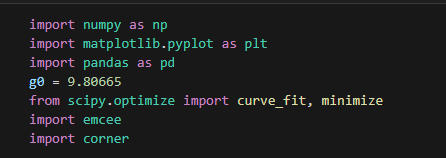
\includegraphics[width=1\linewidth]{FD1.png}
    \caption{前置作業程式碼(1)}
    \label{fig:FD1}
\end{figure}

\indent 在Fig.\ref{fig:FD1}中,我們引入函式庫:
\begin{itemize}
    \item \texttt{numpy} (\texttt{np}): 用於數值運算
    \item \texttt{pandas} (\texttt{pd}): 用於讀取CSV檔案並處理表格數據
    \item \texttt{astropy.constants.g0}: 取得標準重力加速度$g_0$=9.80665$\,m/s^2$
    \item \texttt{scipy.optimize}的\texttt{curve\_fit} 和 \texttt{minimize}: 用來執行數據擬合
    \item \texttt{emcee} 和 \texttt{corner}: 用於貝葉斯MCMC參數估計
\end{itemize}

\clearpage

\begin{figure}[h]
    \centering
    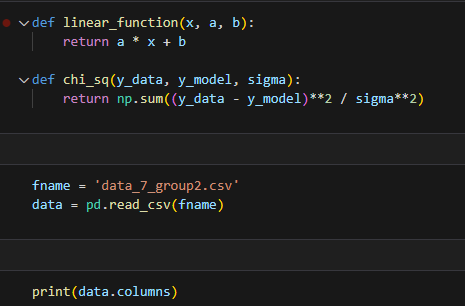
\includegraphics[width=1\linewidth]{FD2.png}
    \caption{前置作業程式碼(2)}
    \label{fig:FD2}
\end{figure}
\indent 定義線性函數$y=ax+b$、卡方檢定函數;並讀取課程提供之CSV檔案,最後輸出欄位名稱。

\begin{figure}[h]
    \centering
    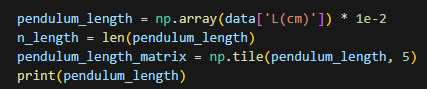
\includegraphics[width=1\linewidth]{FD3.png}
    \caption{前置作業程式碼(3)}
    \label{fig:FD3}
\end{figure}
\indent Fig.\ref{fig:FD3}轉換數據長度單位並把擺長複製五次,於繪圖對應使用,並輸出擺長。

\clearpage

\begin{figure}[h]
    \centering
    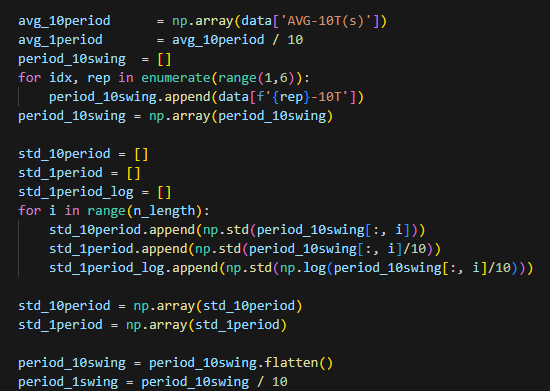
\includegraphics[width=1\linewidth]{FD4.png}
    \caption{前置作業程式碼(4)}
    \label{fig:FD4}
\end{figure}
\begin{figure}[h]
    \centering
    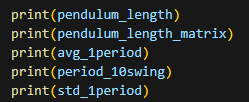
\includegraphics[width=0.5\linewidth]{FD5.png}
    \caption{前置作業程式碼(5)}
    \label{fig:FD5}
\end{figure}
\indent 我們先計算擺動週期:取十次週期求平均,並將1-10T到5-10T取出來並存成5$\times$10陣列,為5次測量的10次週期數據;接著計算標準差,並攤平成一維陣列、轉換單擺週期,最後輸出數值。

\clearpage

\begin{figure}[h]
    \centering
    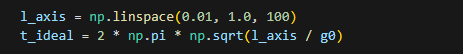
\includegraphics[width=1\linewidth]{FD6.png}
    \caption{前置作業程式碼(6)}
    \label{fig:FD6}
\end{figure}
\indent 產生100個擺長數據並根據公式Eq.\ref{eq:T}計算週期。

\begin{figure}[h]
    \centering
    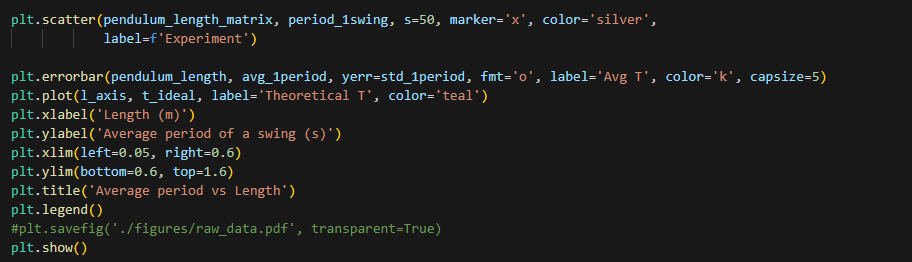
\includegraphics[width=1\linewidth]{FD7.png}
    \caption{前置作業程式碼(7)}
    \label{fig:FD7}
\end{figure}
\indent 繪製單擺實驗數據與理論預測的比較圖表,包含實驗測量數據(銀色x標記)、平均週期與誤差棒(黑色圓點)(顯示每個擺長的平均測量值,並附帶標準差誤差棒,反映測量的不確定性)以及理論預測曲線(藍綠色曲線);設定圖表標籤與範圍,設定x軸為擺長(m),y軸為擺動週期(s),\texttt{plt.legend()} 顯示圖例,區分測量數據、平均值與理論曲線。儲存並顯示圖表。

\clearpage

\subsection{方法一:\texttt{curve\_fit}}
\hfill

\begin{figure}[h]
    \centering
    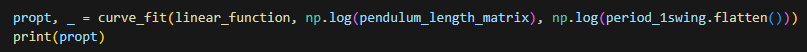
\includegraphics[width=1\linewidth]{curve1.png}
    \caption{\texttt{curve\_fit}程式碼(1)}
    \label{fig:curve_fit1}
\end{figure}
\indent 使用\texttt{curve\_fit}來擬合一條線性函數$\log(T)=a\log(L)+b$;propt[0]為斜率,propt[1]為截距b。

\begin{figure}[h]
    \centering
    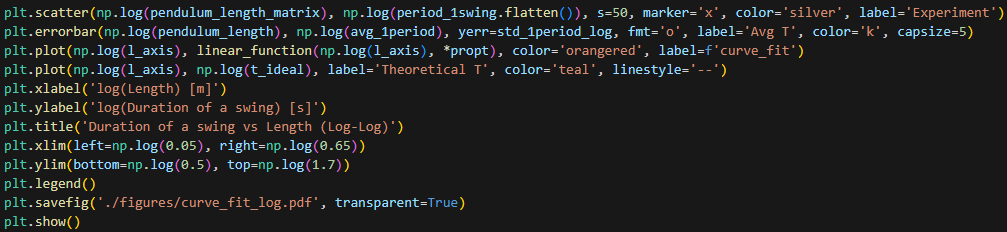
\includegraphics[width=1\linewidth]{curve2.png}
    \caption{\texttt{curve\_fit}程式碼(2)}
    \label{fig:curve_fit2}
\end{figure}
\indent 繪製Log-Log圖,並比較擬合結果與理論值。實驗數據的對數值用銀色交叉符號顯示,error bar使用黑色圓點(如Fig.\ref{fig:curve_fit}右圖)。

\begin{figure}[h]
    \centering
    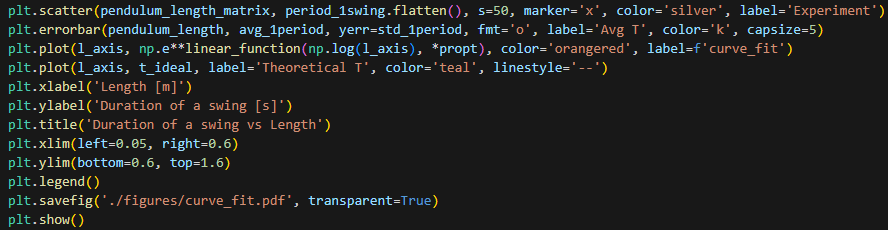
\includegraphics[width=1\linewidth]{curve3.png}
    \caption{\texttt{curve\_fit}程式碼(3)}
    \label{fig:curve_fit3}
\end{figure}
\indent 繪製原始尺度的時間vs.擺長圖,已轉為線性尺度(Fig.\ref{fig:curve_fit}左圖)。

\clearpage

\begin{figure}[h]
    \centering
    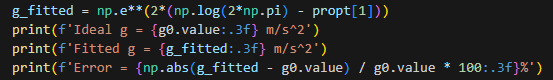
\includegraphics[width=1\linewidth]{curve4.png}
    \caption{\texttt{curve\_fit}程式碼(4)}
    \label{fig:curve_fit4}
\end{figure}
\indent 透過擬合結果估算重力加速度g。最後我們計算之結果$g=9.902\,m/s^2$,與理論的$g_0=9.807\,m/s^2$誤差0.975\%。

\begin{figure}[h]
    \centering
    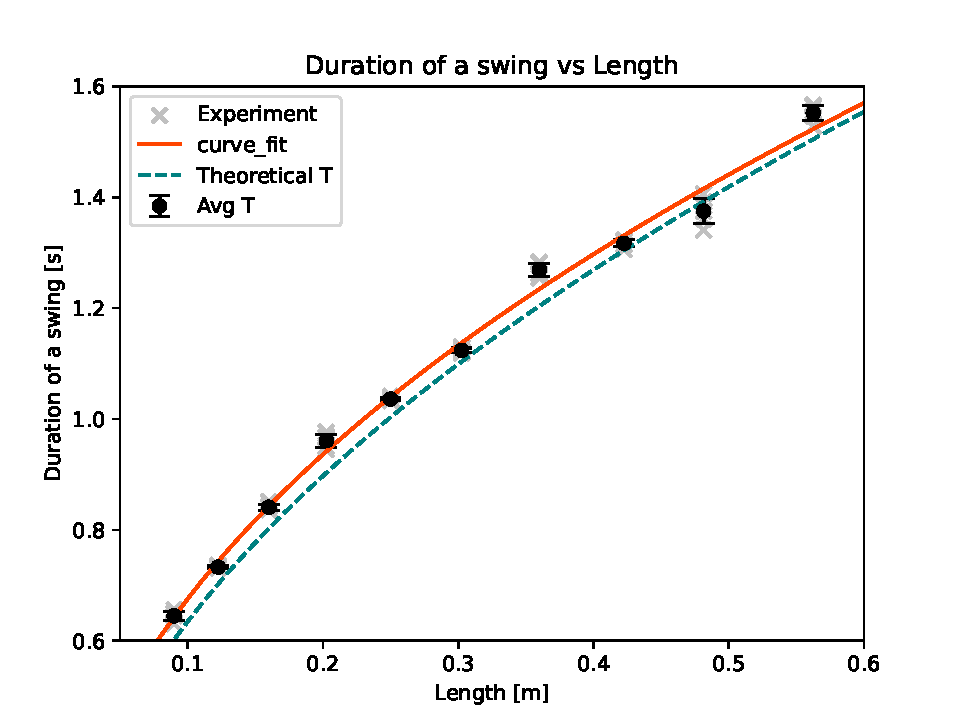
\includegraphics[width=0.45\linewidth]{curve_fit.pdf}
     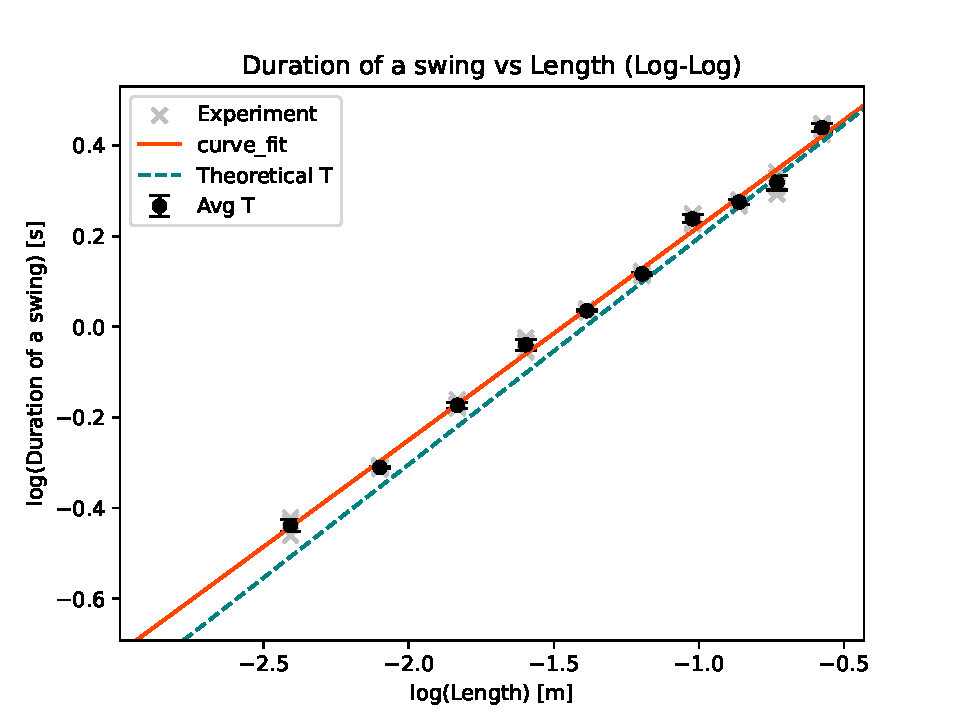
\includegraphics[width=0.45\linewidth]{curve_fit_log.pdf}
    \caption{Enter Caption}
    \label{fig:curve_fit}
\end{figure}

\subsubsection{\texttt{curve\_fit} 數據分析}
\hfill

擺長(Length)與單擺週期(Period)之間的關係,理論上應符合eq.(6)和eq.(7)之公式。

因此,將實驗數據取對數(log-log)後,理論上會呈現線性關係,理論之斜率值為 0.5。

擬合結果的斜率 $\approx0.47$,與理論值 0.50接近。藉由截距項,可以得知對應的g值:$g\approx9.902 \,m/s^2$,與理論值的$g_0 =9.807\,m/s^2$的相對誤差約為 0.975\%,表示此擬合結果具有高準確度。此外,透過圖表也可以看出擬合曲線與實驗平均值相符,顯示模型與實測結果大致具有一致性。雖然整體擬合結果看起來大致上符合預期,但是根據圖表可以看出,在較短擺長處部分與理論曲線之間有相對之下較為顯著的差距。這可能是由於較短襬長處週期測量誤差比例較大,抑或者是運動過程非理想擺運動所造成的偏差有關,也可能是由於擺幅較大、擺錘起始角度有落差或者是其他人為誤差所造成的。

\subsubsection{\texttt{curve\_fit} 誤差討論}
\hfill

擬合斜率偏差:擬合斜率為0.471,而斜率之理論值為0.5,相對誤差約為 5.8\%。

進一步討論誤差來源:
\begin{enumerate}
    \item 缺乏誤差加權:\\預設情況下,\texttt{curve\_fit} 將所有資料點視為同樣可靠,不會根據不同資料點的誤差大小進行加權。因此如果有某些點的測量誤差較大,就會對擬合產生過度的影響。
    \item 初始值選擇:\\ 雖然 \texttt{curve\_fit} 本身會自動選擇初始值,但是在複雜模型中,若初始猜測與真實值差太多,可能導致擬合陷入局部極小值而非全域最佳解、擬合失敗或收斂很慢等情形發生。
    \item 異常值影響:\\最小平方法對異常值敏感,單一點偏差過大就有可能對整體擬合結果造成顯著影響。透過平均與標準差處理,以及觀察殘差圖與誤差棒,可以初步確認資料穩定性良好。
\end{enumerate}

\subsection{方法二:Least square fitting}
\hfill

\begin{figure}[h]
    \centering
    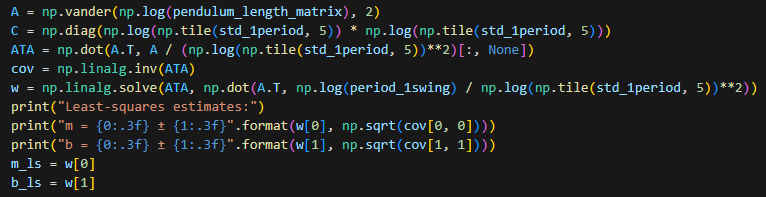
\includegraphics[width=1\linewidth]{LS1.png}
    \caption{LS程式碼(1)}
    \label{fig:LS1}
\end{figure}
\indent 最小二乘法擬合np.vander$(x, 2)$產生 Vandermonde矩陣,對應線性模型$\log T=m\log L+b$。參數如下:\\
\begin{itemize}
    \item C是對角矩陣,考慮log週期的誤差。
    \item ATA = $A^T$ $C^{-1}A$是加權最小二乘法的矩陣。
    \item cov = np.linalg.inv(ATA) 計算參數的不確定性(共變異矩陣)。
    \item $w = [m, b]$ 是最小二乘法解出來的參數。
\end{itemize}

\clearpage

\begin{figure}[h]
    \centering
    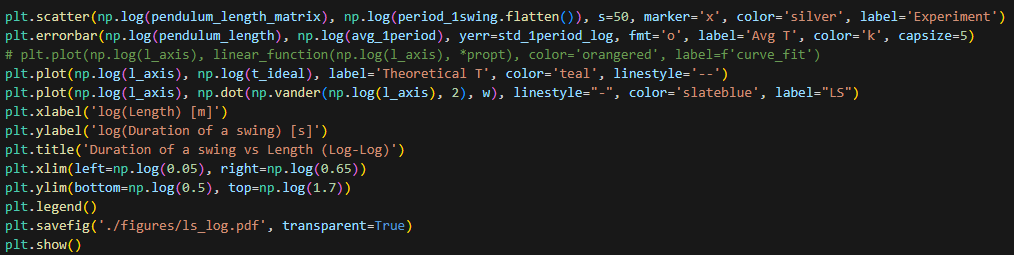
\includegraphics[width=1\linewidth]{LS2.png}
    \caption{LS程式碼(2)}
    \label{fig:LS2}
\end{figure}
\indent Log-Log圖,檢查LS擬合曲線是否與理論值相符;銀色交叉符號為實際對數值,黑色圓點表error bar(如Fig.\ref{fig:LS}
右圖)。

\begin{figure}[h]
    \centering
    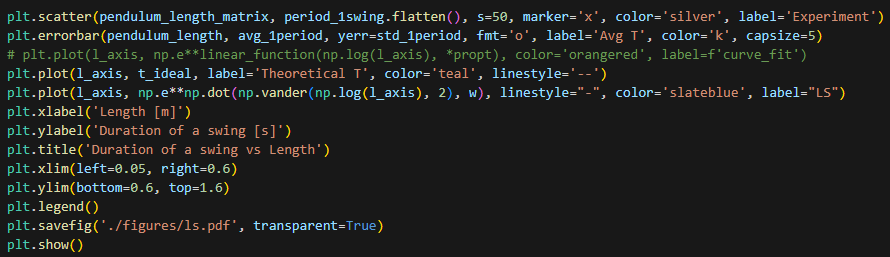
\includegraphics[width=1\linewidth]{LS3.png}
    \caption{LS程式碼(3)}
    \label{fig:LS3}
\end{figure}
\indent 原始尺度圖,藍色實線(LS擬合)與理論曲線(虛線)做比較,檢查擬合效果(Fig.\ref{fig:LS}左圖)。

\begin{figure}[h]
    \centering
    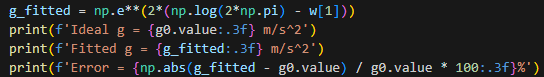
\includegraphics[width=1\linewidth]{LS4.png}
    \caption{LS程式碼(4)}
    \label{fig:LS4}
\end{figure}

最後我們計算之結果$g=9.969\,m/s^2$,與理論的$g_0=9.807\,m/s^2$誤差1.660\%

\clearpage

\begin{figure}[h]
    \centering
    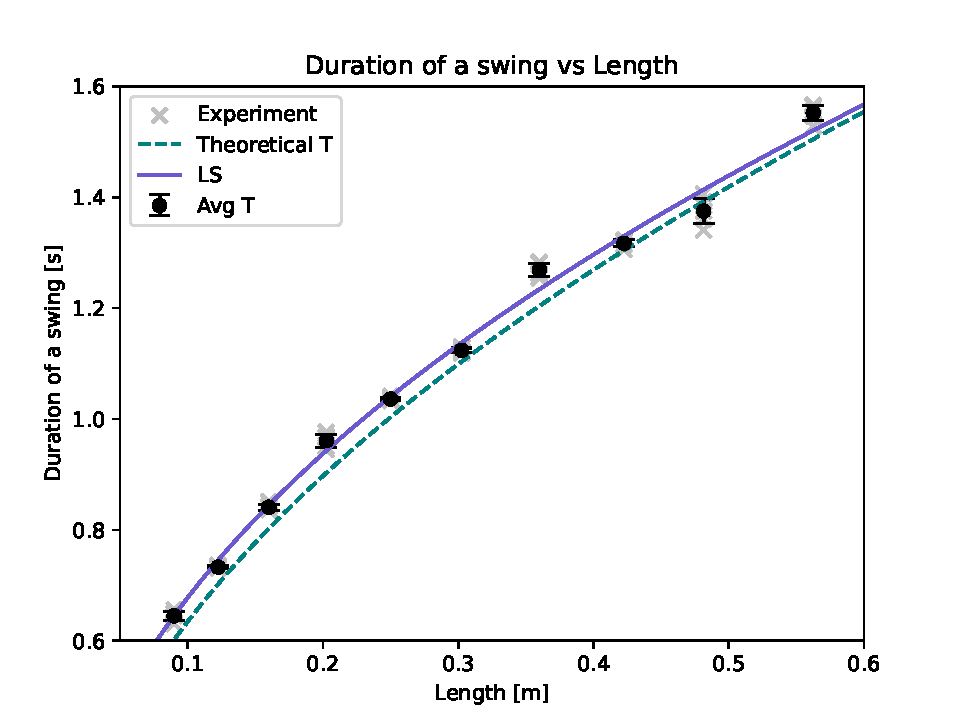
\includegraphics[width=0.45\linewidth]{ls.pdf}
    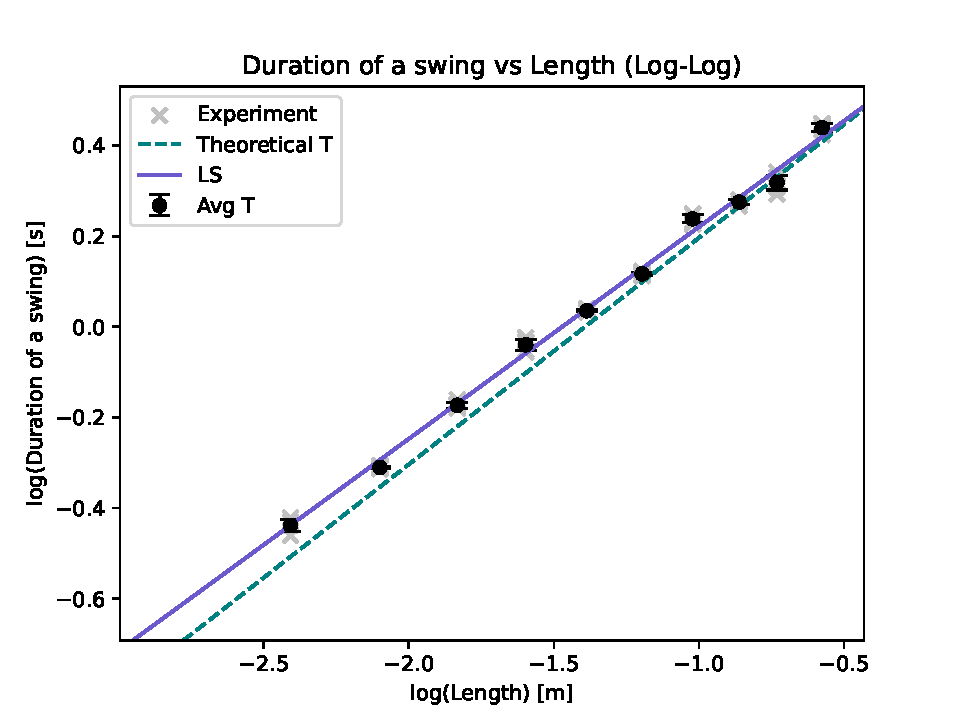
\includegraphics[width=0.45\linewidth]{ls_log.pdf}
    \caption{Enter Caption}
    \label{fig:LS}
\end{figure}

\subsubsection{LS 數據分析}
\hfill

此部分使用了加權最小平方法(Weighted Least Squares),考慮每筆資料的誤差(標準差)作為權重,使得誤差較小的數據點在擬合中影響更大,進而嘗試提升實驗結果的準確度而確保不過度受到誤差大的數距點影響。

計算後的擬合參數為:
\begin{itemize}
    \item 斜率:$m=0.485\pm0.012$
    \item 截距:$b=0.668\pm0.008$
\end{itemize}

由上方數據可以看出,資料整體仍趨近於理論模型,落差較小。尤其式斜率數值接近斜率理論值0.5,即能代表擺長與週期的平方關係符合、成立。
擬合後推算出的g值為$g = 9.969\,m/s^2$,與理論的$g_0 = 9.807\,m/s^2$誤差1.660\%。

與先前\texttt{curve\_fit}得到誤差(0.975\%)相比,雖然Least square fitting算出的g值誤差相對較大,但仍屬於合理範圍內,故顯示模型仍然準確合理。從圖表也可得知實驗數據(黑色點與誤差條)整體呈現隨擺長增加則週期增加的趨勢,符合理論公式eq.(6)的非線性曲線(虛線)。

\subsubsection{LS 誤差討論}
\hfill

Least square fitting將每筆資料的測量不確定度納入考量,給予誤差小的點較高的權重,降低誤差較大的點對擬合結果的影響。但本次擬合中所得所得誤差相較之下較高,可能原因如下:

\begin{enumerate}
    \item 誤差估計不穩定:\\資料誤差來源主要來自每筆資料標準差,如果資料的數量有限,使標準差本身不夠穩定,就有可能造成權重設置不準確進而導致誤差。
    \item 誤差分佈未完全服從高斯分佈:\\最小平方法假設誤差為常態分佈,但如果實際誤差分佈有偏態的情形,則加權擬合效果可能因此受限。
    \item 異常值影響未修正:\\雖然LS fitting對誤差小的點給予較高權重,但依舊會受到異常值影響,因此可以搭配異常值偵測或穩健迴歸。
\end{enumerate}

此外,理論上從截距推算重力加速度時,任何的微小誤差都會被指數放大。例如截距b之誤差$\pm0.008$,經指數與平方運算後,算出 g值的誤差為 1.6\%,反映出了非線性取線之誤差放大效應。因此若是要讓回推得出的g值更加準確,則需減少截距的不確定度,抑或是嘗試改用其他能更穩定的方法。


\clearpage

\subsection{方法三:$\chi^2$ fitting}
\hfill

\begin{figure}[h]
    \centering
    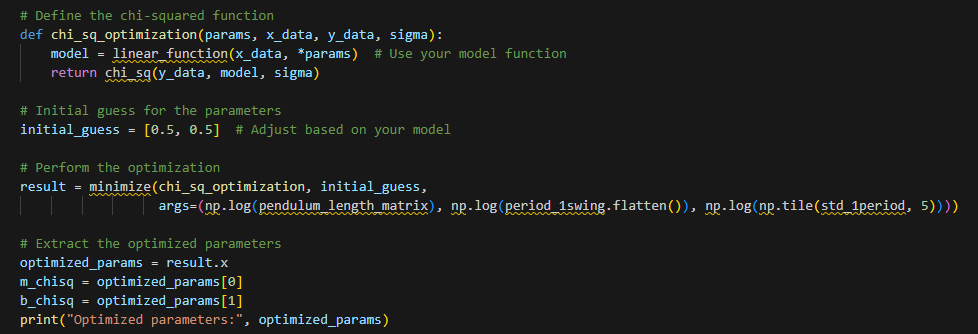
\includegraphics[width=1\linewidth]{chi1.png}
    \caption{$\chi^2$ fitting程式碼(1)}
    \label{fig:chi1}
\end{figure}
\begin{figure}[h]
    \centering
    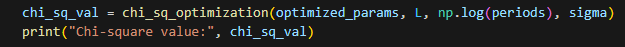
\includegraphics[width=1\linewidth]{chi5.png}
    \caption{$\chi^2$ fitting程式碼(2)}
    \label{fig:chi5}
\end{figure}
Fig.\ref{fig:chi1}是先定義chi-squared function,並定義:\\
params為我們要最佳化的參數(直線之斜率或截距);\\
$x\_data$和$y\_data$為輸入數據;\\
sigma為測量不確定性;\\
linear\_function($x\_data$, \*params)為一條直線;($y=ax+b$)\\
chi\_sq(y\_data, model, sigma)為計算$\chi^2$。\\
\indent 接著設定初始參數,先猜測m=0.5、b=0.5;並進行最小化$\chi^2$。\\
\indent 而因為實驗要求擬合擺動週期與擺長的對數關係,所以需取對數,使其變線性關係(詳情見預習問題1、2)即可求得a、b。\\
\indent 最後把最佳化後的m、b,和$\chi^2$值顯示出來。\\
\indent 最終輸出結果:\\
Optimized parameters: [0.48023142 0.79271392]\\
Chi-square value: 0.15251356436613928


\begin{figure}[h]
    \centering
    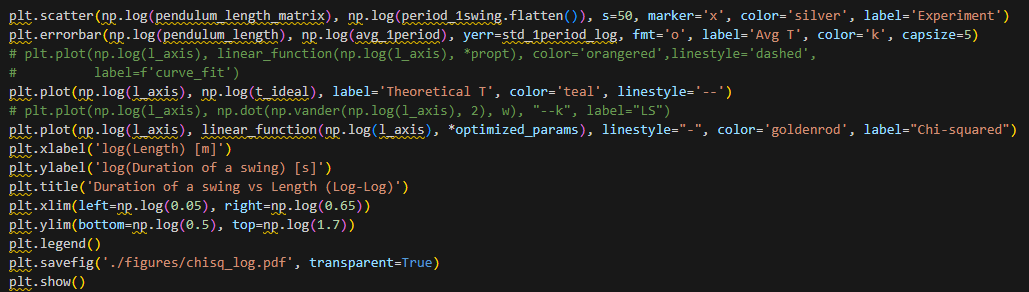
\includegraphics[width=1\linewidth]{chi2.png}
    \caption{$\chi^2$ fitting程式碼(3)}
    \label{fig:chi2}
\end{figure}

Fig.\ref{fig:chi2}使用\texttt{plt.scatter()}繪製實驗數據點;x軸為擺長取對數;y軸為單次擺動週期取對數。利用交叉符號點出個別數據點。\\
\indent 接著繪出理論曲線和$\chi^2$擬合的曲線,並設定座標軸與標題及範圍;結果為Fig.\ref{fig:chi_sq}右圖。


\begin{figure}[h]
    \centering
    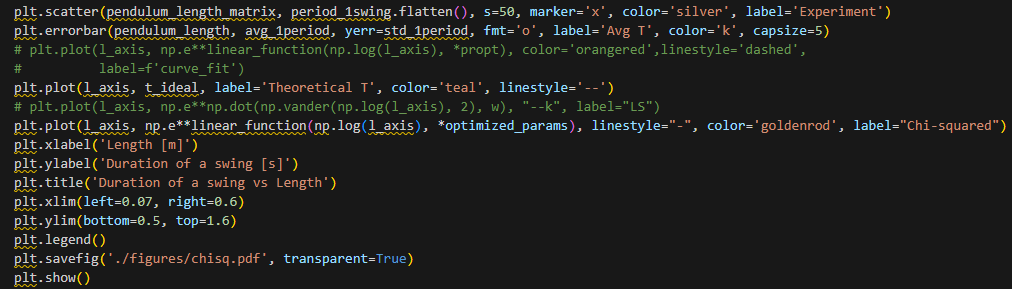
\includegraphics[width=1\linewidth]{chi3.png}
    \caption{$\chi^2$ fitting程式碼(4)}
    \label{fig:chi3}
\end{figure}
\indent Fig.\ref{fig:chi3}繪製擺長與擺動週期的關係圖,但和上部分的對數-對數圖不同,這次是線性尺度。\\
\indent 令x軸為擺長、y軸為擺動週期,用銀色交叉符號標出實驗數據,並繪出error bar(使用黑色圓點,表測量之不確定性);最後劃出理論曲線和$\chi^2$理論曲線與我們擬合出的結果(Fig.\ref{fig:chi_sq}左圖)。

\begin{figure}[h]
    \centering
    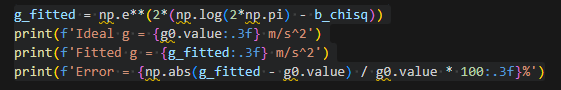
\includegraphics[width=1\linewidth]{chi4.png}
    \caption{$\chi^2$ fitting程式碼(5)}
    \label{fig:chi4}
\end{figure}

Fig.\ref{fig:chi4}透過$\chi^2$擬合的結果估算重力加速度$g$,並和理論值($g_0$)比較。\\
\indent 計算方法參考預習問題1、2推導之公式。
最後我們計算之結果$g=9.969\,m/s^2$,與理論的$g_0=9.807\,m/s^2$誤差1.660\%。

\begin{figure}[h]
    \centering
    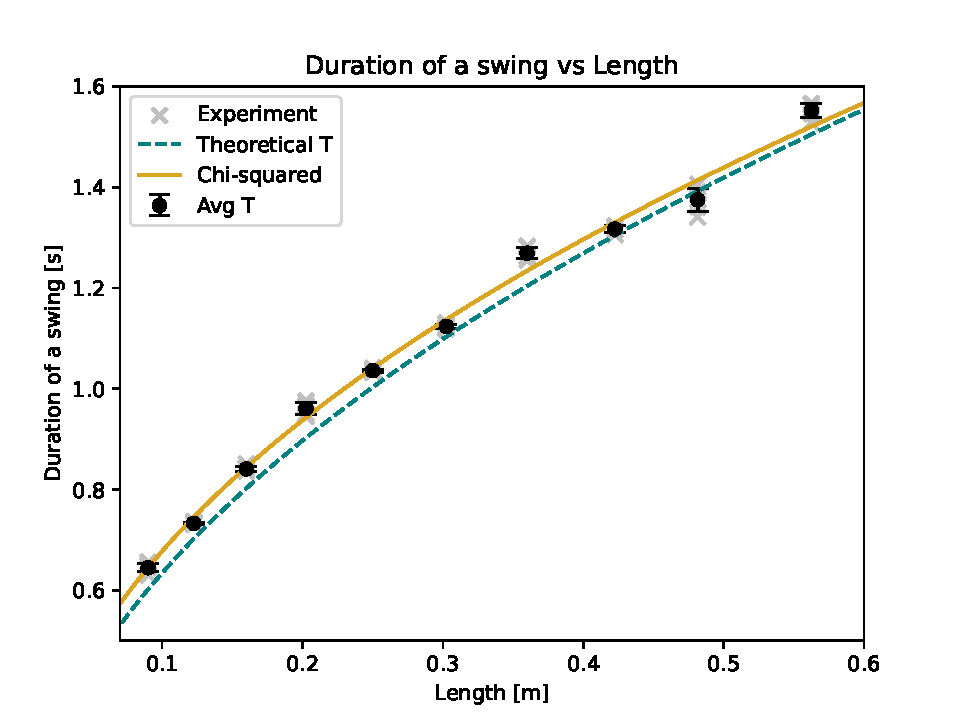
\includegraphics[width=0.45\linewidth]{chisq.pdf}    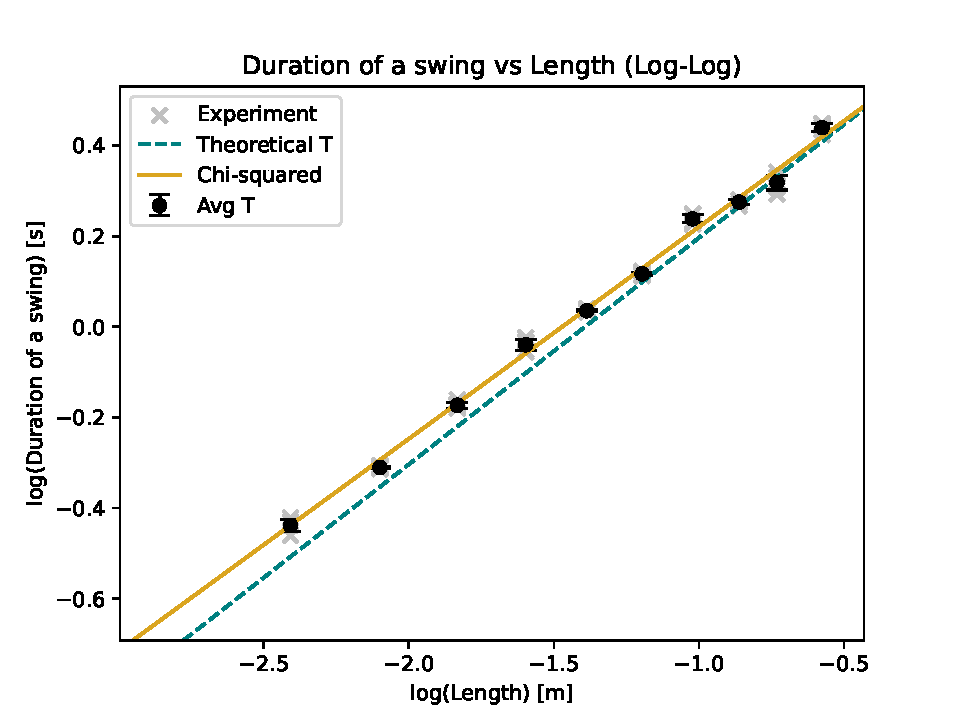
\includegraphics[width=0.45\linewidth]{chisq_log.pdf}
    \caption{$\chi^2$ 擬合結果(左圖為線性擬合;右圖為對數擬合)}
    \label{fig:chi_sq}
\end{figure}

\clearpage

\begin{figure}[h]
    \centering
    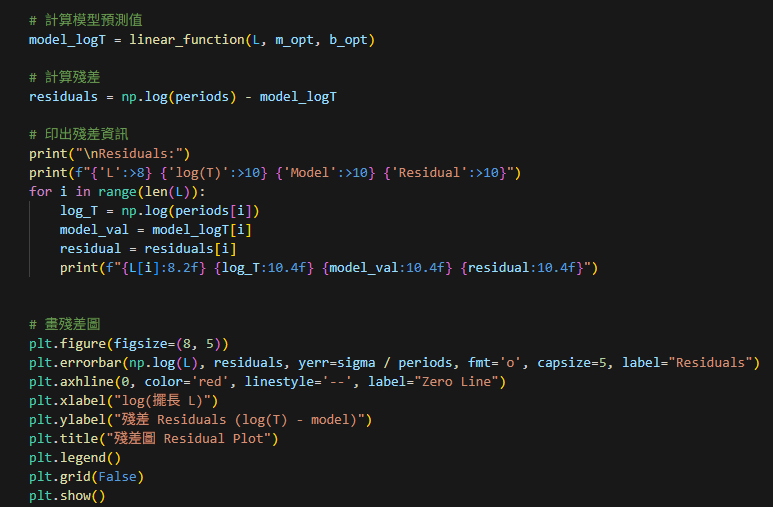
\includegraphics[width=1\linewidth]{chi6.png}
    \caption{$\chi^2$ fitting程式碼(6)}
    \label{fig:chi6}
\end{figure}

\indent Fig.\ref{fig:chi6}為計算殘差的標準差,詳情見圖上程式碼註解,我們計算出之各數據殘差為:
\renewcommand{\arraystretch}{1.5}
\begin{center}
\begin{tabular}{|c|c|c|c|}
    \hline
    擺長L(cm)& log(T) & Model & Residual \\
    \hline
    56.25&2.7492&2.7280&0.0212 \\
    \hline
    48.15&2.6210&2.6533&-0.0322 \\
    \hline
    42.25 &2.5810&2.5905&-0.0095 \\
    \hline
    36.00 &2.5518&2.5136&0.0382 \\
    \hline
    30.25 &2.4186&2.4301&-0.0115 \\
    \hline
    25.00 &2.3351&2.3385&-0.0035 \\
    \hline
    20.25&2.2460&2.2373&0.0087\\
    \hline
    16.00&2.1294&2.1242&0.0052\\
    \hline
    12.25&1.9961&1.9959&0.0001\\
    \hline
    9.00&1.8421&1.8479&-0.0058\\
    \hline
\end{tabular}
\end{center}

\clearpage

\indent 殘差圖如下:

\begin{figure}[h]
    \centering
    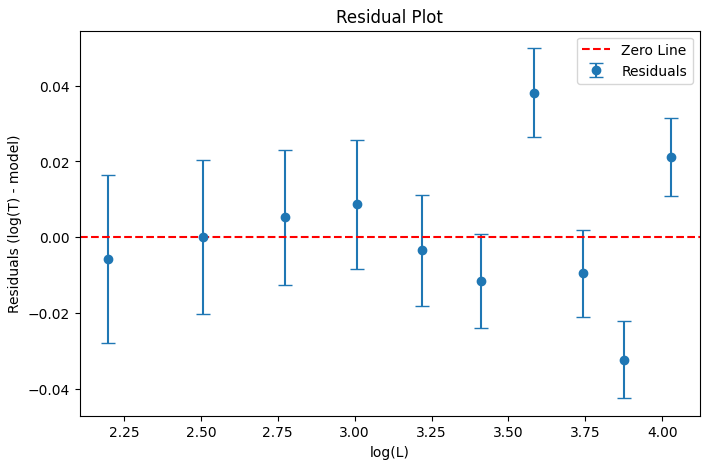
\includegraphics[width=1\linewidth]{aaaaaaaaaaaaaaaa.png}
    \caption{殘差圖}
    \label{fig:chiB}
\end{figure}

%CHI
\subsubsection{$\chi^2$ fitting 數據分析}
\hfill

\indent 從Fig.\ref{fig:chi_sq}左圖「擺動週期與擺長的關係」可見,實驗數據(黑色點與誤差條)整體呈現隨擺長增加而週期增加的趨勢,符合理論公式eq.(6)的非線性曲線(虛線)。\\
\indent 而理論曲線與部分實驗數據點有些許偏差,進一步使用Chi-square擬合(橘線)進行資料擬合,而我們得到最佳化的參數為:
   $ m=0.4802$;$b=0.7927$\\
\indent 其中b略大於理論值之0.5,推測來自實驗時的空氣阻力、測量誤差等非理想條件。\\
\indent 計算之$\chi^2$值為0.1525。\\
此值遠小於自由度,於誤差討論和問題討論第一題詳細討論;自由度為$N-2=8$:\\
\indent $\chi^2 \approx 0.1525$\\
\indent $\chi_{reduced}^2=\frac{0.1525}{8} \approx 0.0019$\\

\indent Fig.\ref{fig:chi_sq}右圖為相同資料轉換為對數座標下的結果。理論預測為一條斜率為0.5之值線,而Chi-square擬合同樣顯示與實驗資料的對數變化趨勢更一致,進一步證實擬合品質。
\indent 見Fig.\ref{fig:chiB},殘差圖呈現資料點約略隨機分佈於零線上下,而無特定趨勢。在$\log(L)$=3.5左右時較大,推測原因為在測量數據時有較大的誤差(人工因素等等),而形成較大的殘差。

\subsubsection{$\chi^2$ fitting 誤差討論}
\hfill

\indent 由於我們計算出的$\chi^2$值相對非常小,可能有以下情況:\\

\begin{enumerate}
    \item 誤差估計可能偏大:\\
    若error bar過大,導致$\chi^2$值過低,即使模型不正確也會看似完美。
    \item 資料波動小:\\若每次實驗測得的擺動週期變異不大(數據高度集中),也可能產生偏低的$\chi^2$值。
    \item 過度擬合潛在可能:\\擬合模型使用自由參數調整得非常貼合資料點,但未必具有物理意義。此情況下,雖然卡方值低,但模型的泛化能力下降。
\end{enumerate}

\indent 可透過以下方法改進:
\begin{enumerate}
    \item 重新估算error bar:\\採每個擺長點多次重複測量週期,計算平均與標準差作為error bar。
    \item 進行殘差分析:\\檢視實驗值與擬合值之間的差異(殘差),若呈現隨擺長有系統偏移,可能代表模型還有未考慮的物理因素(如空氣阻力、繩長非理想、非簡諧運動等),可據此進行修正。
\end{enumerate}


\clearpage

\subsection{方法四:MCMC fitting}
\hfill

\begin{figure}[h]
    \centering
    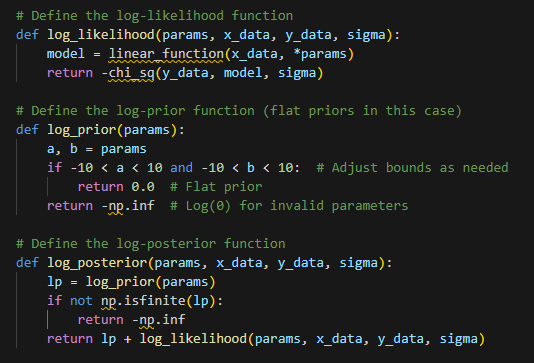
\includegraphics[width=1\linewidth]{MCMC1.png}
    \caption{MCMC程式碼(1)}
    \label{fig:MCMC1}
\end{figure}

這部分是利用MCMC(Markov Chain Monte Carlo)取樣,建立對數後驗分佈函數,並定義三個MCMC取樣所需之函數:
\begin{enumerate}
    \item log-likelihood
    \item log-prior
    \item log-posterior
\end{enumerate}
\indent 首先先定義log-likelihood,參數如下:
\begin{itemize}
    \item params:模型的參數$(a,b)$(線性模型之斜率與截距)
    \item $x\_data$:自變數
    \item $y\_data$:因變數
    \item sigma:測量誤差
\end{itemize}
\indent 先使用linear\_function(x\_data, \*params)計算模型預測值;接著計算出$\chi^2$,再來由於likelihood function $\mathcal{L}$通常與$e^{\frac{-\chi^2}{2}}$成正比,可取對數得其值。\\
\indent 最後回傳log-likelihood作為評估參數的可能性。\\
\indent 再來利用Flat Prior設計log-prior,表示我們對參數$(a,b)$的先驗知識。\\
\indent 最後定義log-posterior,即為貝葉斯定理。

\begin{figure}[h]
    \centering
    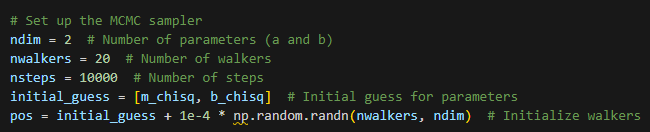
\includegraphics[width=1\linewidth]{MCMC2.png}
    \caption{MCMC程式碼(2)}
    \label{Fig.MCMC2}
\end{figure}
\begin{figure}[h]
    \centering
    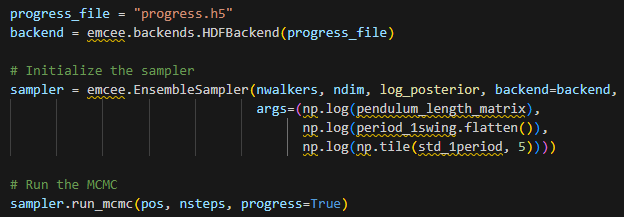
\includegraphics[width=1\linewidth]{MCMC3.png}
    \caption{MCMC程式碼(3)}
    \label{fig:MCMC3}
\end{figure}

\indent Fig.\ref{Fig.MCMC2}和Fig.\ref{fig:MCMC3}是開始使用MCMC進行參數的擬合。\\
\indent 首先先設定MCMC參數與初始點(兩個參數、20個行走者、每個行走者執行1000步),並在初始化MCMC採樣器後執行。

\clearpage

\begin{figure}[h]
    \centering
    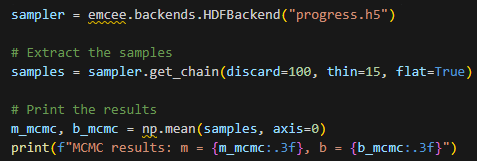
\includegraphics[width=1\linewidth]{MCMC4.png}
    \caption{MCMC程式碼(4)}
    \label{fig:MCMC4}
\end{figure}

\begin{figure}[h]
    \centering
    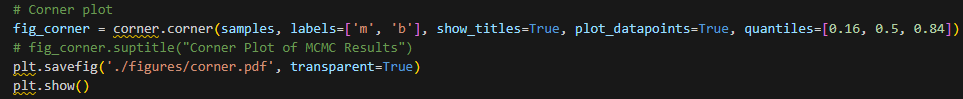
\includegraphics[width=1\linewidth]{MCMC5.png}
    \caption{MCMC程式碼(5)}
    \label{fig:MCMC5}
\end{figure}
\indent Fig.\ref{fig:MCMC4}和Fig.\ref{fig:MCMC5}目的是讀取MCMC的取樣結果並分析參數的後驗分佈,最後繪製成圖。\\
\indent 提取MCMC採樣點部分的參數解釋:\\
\begin{itemize}
    \item $discard=100$為丟棄前100步,確保MCMC收斂後樣本才被使用。
    \item $thin=15$每15步取一個樣本。
    \item flat=True將所有行走者的樣本合併成一個長列表。
\end{itemize}
\indent 最後計算MCMC擬合出的最佳參數(斜率m與截距b)。

\clearpage

\begin{figure}[h]
    \centering
    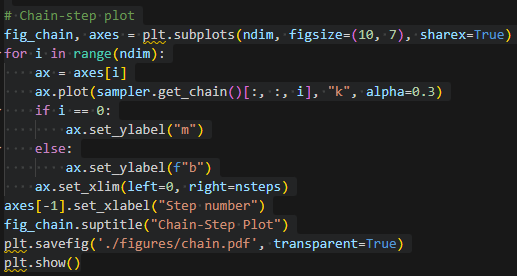
\includegraphics[width=1\linewidth]{MCMC6.png}
    \caption{MCMC程式碼(6)}
    \label{fig:MCMC6}
\end{figure}

\indent 此為診斷MCMC計算後的工具之一(Fig.\ref{fig:IDK})。

\begin{figure}[h]
    \centering
    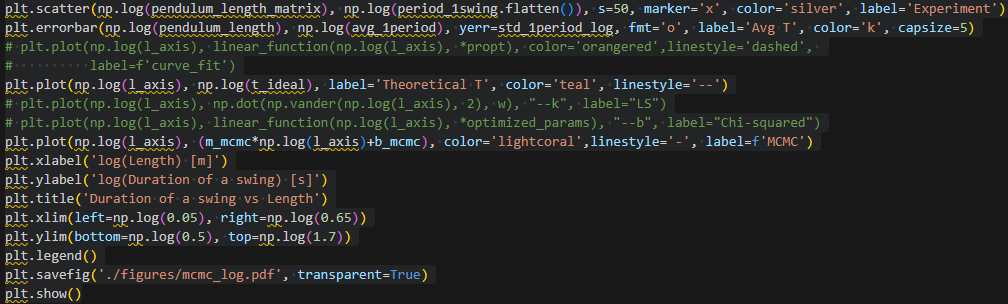
\includegraphics[width=1\linewidth]{MCMC7.png}
    \caption{MCMC程式碼(7)}
    \label{fig:MCMC7}
\end{figure}

\indent 此段為MCMC的擬合結果(對數尺度),繪製出對數尺度的實驗數據與MCMC擬合曲線(為Fig.\ref{MCMC}右圖)。

\clearpage

\begin{figure}[h]
    \centering
    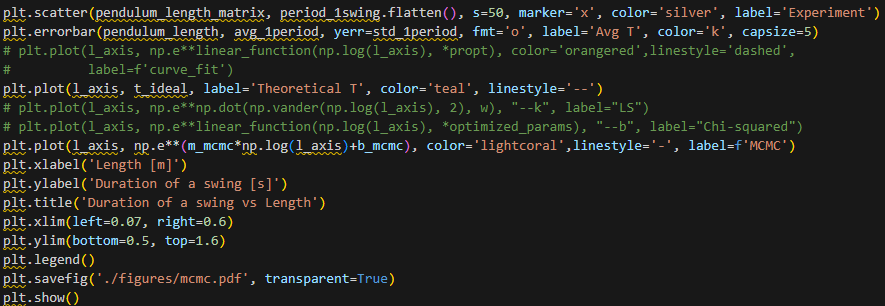
\includegraphics[width=1\linewidth]{MCMC8.png}
    \caption{MCMC程式碼(8)}
    \label{fig:MCMC8}
\end{figure}

\indent 此段為MCMC的擬合結果(線性尺度),繪製出線性尺度的實驗數據與MCMC擬合曲線(為Fig.\ref{MCMC}左圖)。

\begin{figure}[h]
    \centering
    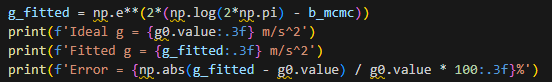
\includegraphics[width=1\linewidth]{MCMC9.png}
    \caption{MCMC程式碼(9)}
    \label{fig:MCMC9}
\end{figure}

最後利用MCMC方法擬合得到$g=9.887\,m/s^2$,與理論的$g_0=9.807\,m/s^2$誤差0.823\%。


\begin{figure}[h]
    \centering
    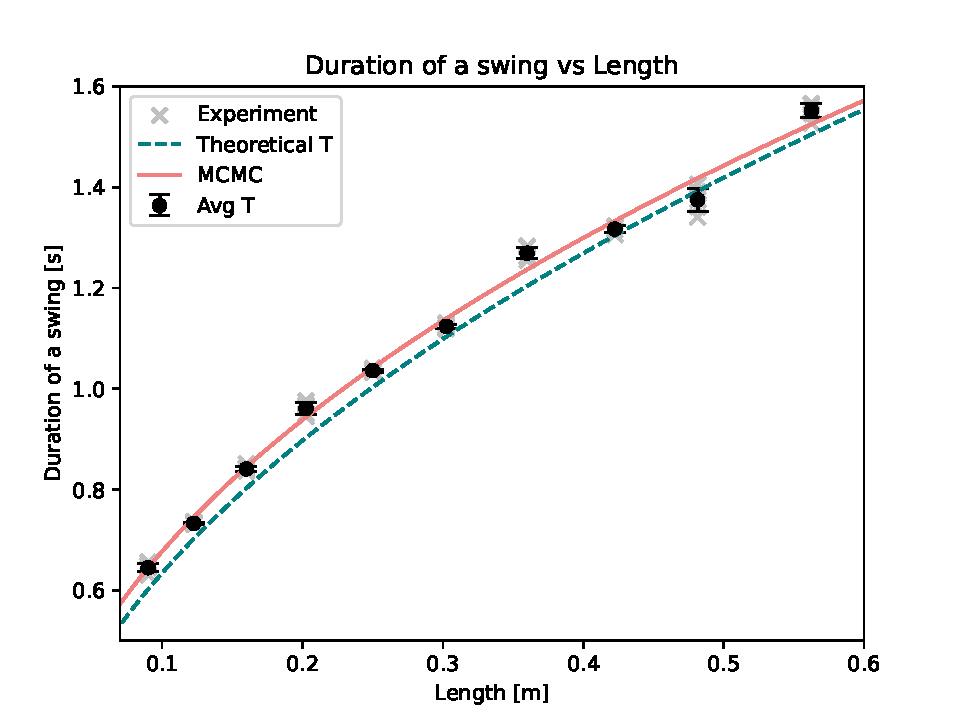
\includegraphics[width=0.45\linewidth]{mcmc.pdf}
    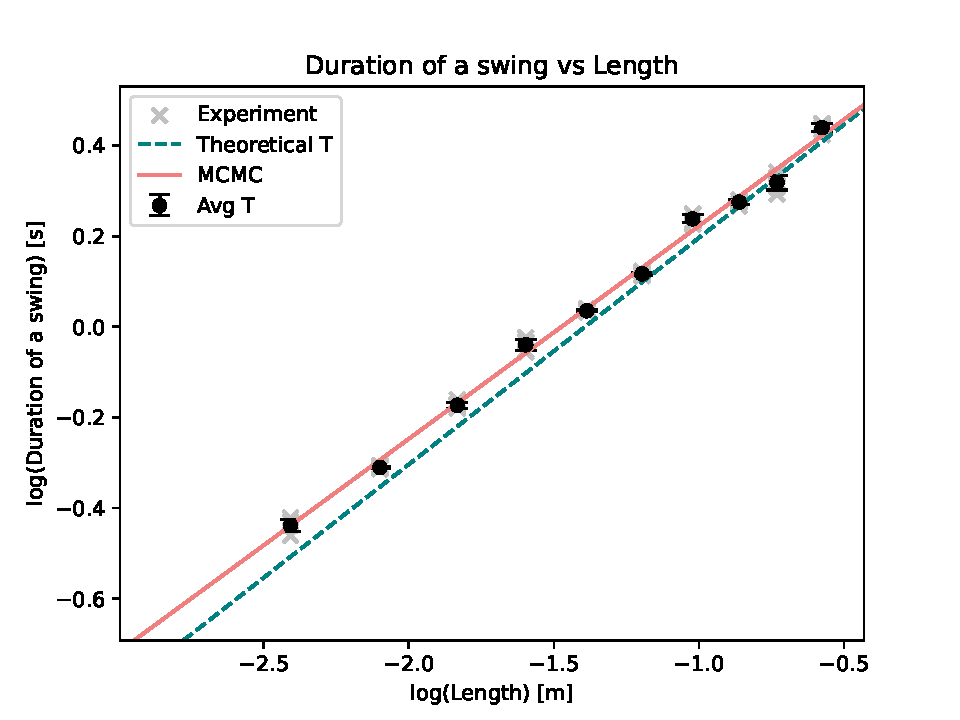
\includegraphics[width=0.45\linewidth]{mcmc_log.pdf}
    \caption{MCMC擬合結果(左圖為線性擬合;右圖為對數擬合)}
    \label{MCMC}
\end{figure}

\clearpage

\begin{figure}[h]
    \centering
    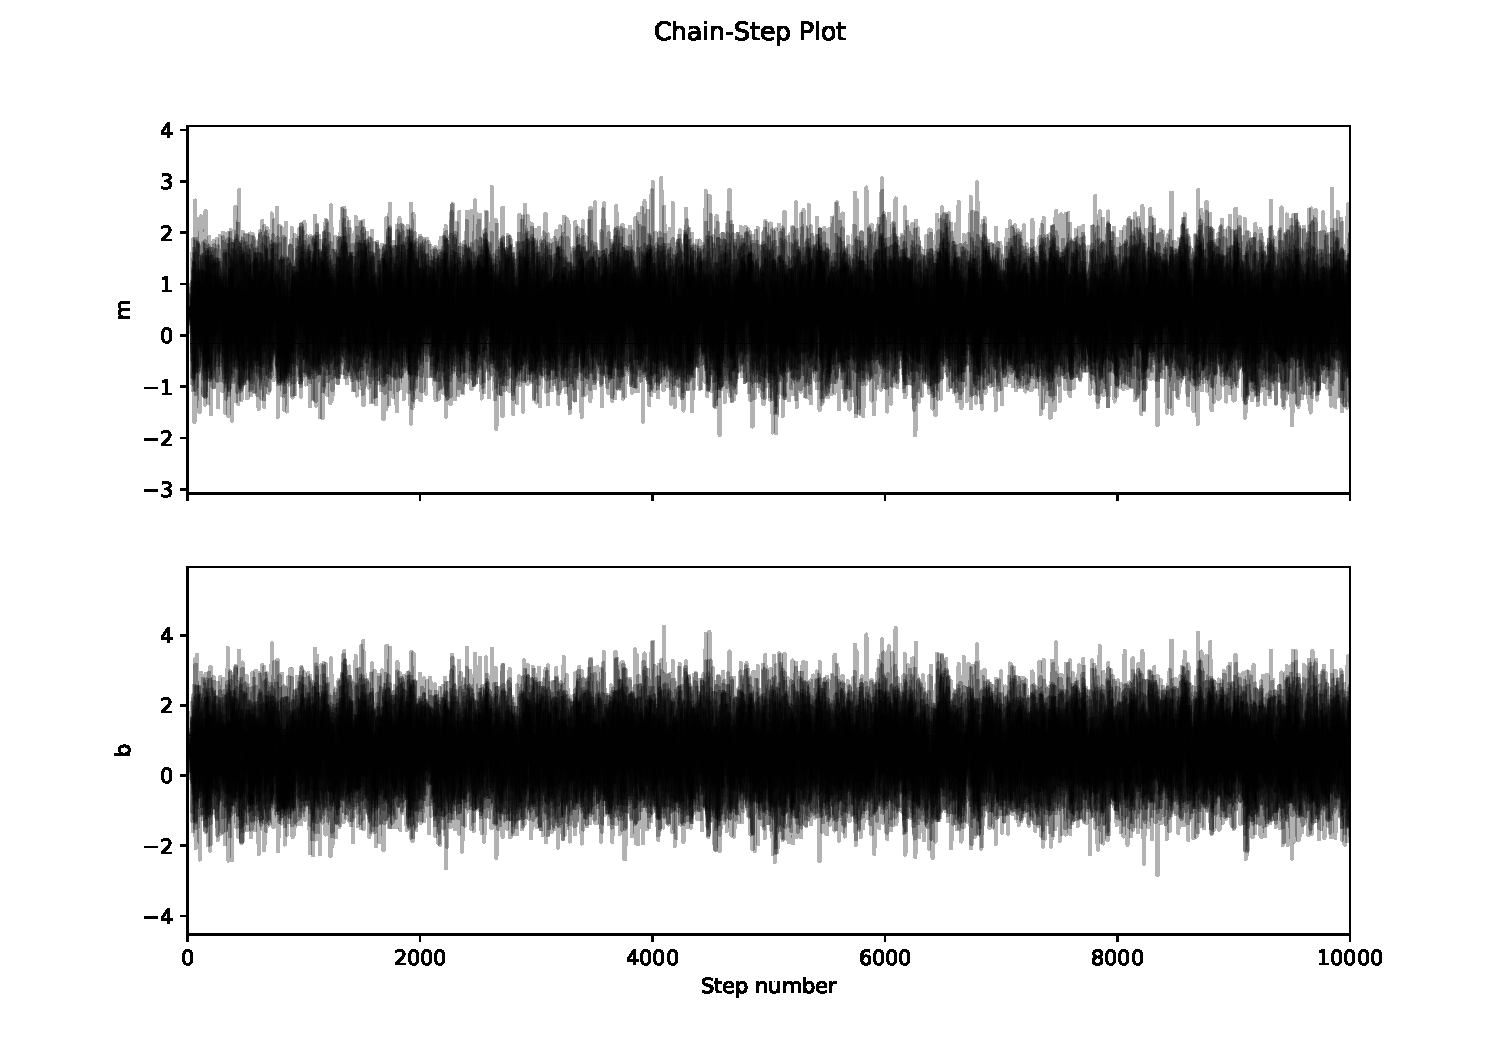
\includegraphics[height=6.5cm]{chain.pdf}
    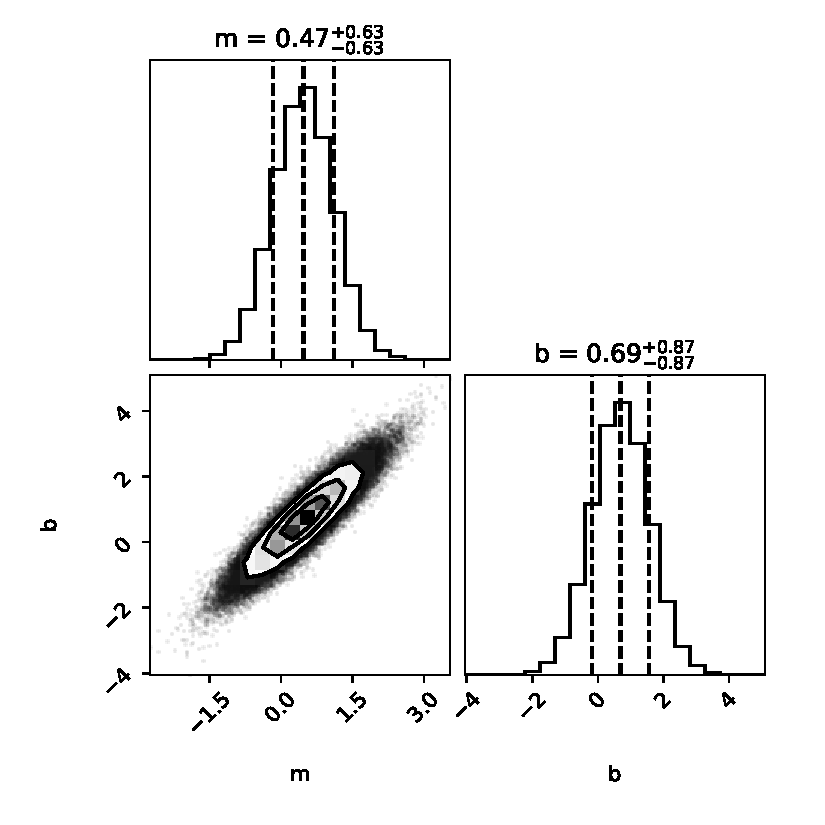
\includegraphics[height=6.5cm]{corner.pdf}
    \caption{Chain-step plot and posterior corner plot}
    \label{fig:IDK}
\end{figure}

%MCMC
\subsubsection{MCMC fitting 數據分析}
\hfill

\indent 如Fig.\ref{MCMC}所示,我們使用另一種方法--MCMC(馬可夫鏈蒙地卡羅)方法做非線性擬合;左圖為線性尺度下的擺長與週期關係,右圖則為對數尺度。\\
\indent MCMC擬合結果(紅線)整體貼合實驗點,與實驗error bar(黑色)一致性良好;相較於理論曲線(虛線),MCMC 模型更能捕捉到實驗數據的微小偏差,尤其在短擺長處擁有更高的吻合度,可能是因為誤差在小擺長處較小,因此權重較大,MCMC 更傾向貼近這些資料點。\\
\indent 在對數-對數圖中,MCMC擬合同樣呈現高度線性,與實驗數據的對數趨勢相符,強化了模型合理性。\\
\indent MCMC不僅給出最佳擬合參數,也能產生參數的後驗分佈,進一步評估其不確定性,使整體擬合更具統計意義,因此我們生成Fig.\ref{fig:IDK}來驗證其擬合解果的可靠性。\\
\indent 在左圖中,兩條鏈分別對應參數m與b的歷程變化,顯示出已達到穩定波動狀態,無明顯飄移或趨勢,表示馬可夫鏈已充分混合並收斂,擬合過程穩定。\\
\indent 右圖為後驗分佈圖,說明參數的不確定性已被資料良好約束。聯合分佈圖中呈現出輕微正相關的橢圓形,亦符合物理模型中擬合參數可能的耦合特性。

\subsubsection{MCMC fitting 誤差討論}
\hfill

\indent 誤差可能來自:
\begin{enumerate}
    \item 參數不確定性來源:\\MCMC 本身會輸出參數的機率分佈,若分佈過寬,代表數據不足以嚴格約束模型;反之若過窄,可能暗示模型過於自信,未考慮潛在系統誤差。
    \item 模型選擇的依賴性:\\MCMC 依賴於設定的模型形式(如冪次關係),若模型假設本身有偏誤,則即使後驗收斂良好,也可能是「錯模型的好擬合」。
    \item error bar可信度影響擬合精度:\\若誤差估計不足(如未反映實驗者反應時間、系統延遲等),會使後驗分佈過窄,導致參數誤判或過度擬合。
\end{enumerate}

\clearpage

\indent 改善的方法:
\begin{enumerate}
    \item 加入參數後驗分佈圖與可信區間:\\展示如$a,b$的後驗分佈,可更具體呈現參數的不確定性,也能對比理論值是否落在可信區間內。
    \item 提升誤差估計的可靠性:\\以每個擺長點進行多次測量(取平均與標準差),減少系統誤差未反映於$\sigma$的問題。
\end{enumerate}



\subsection{比較不同方法}
\hfill

\begin{figure}[h]
    \centering
    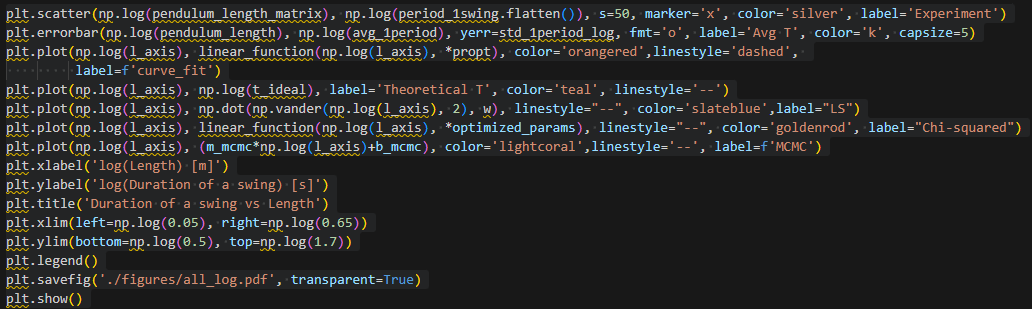
\includegraphics[width=1\linewidth]{CAM1.png}
    \caption{比較不同方法\-程式碼(1)}
    \label{fig:CAM1}
\end{figure}

\indent 最後,我們比較每個方法的差異,分別繪製出最小平方法、卡方檢定、MCMC方法的線性擬合結果比較;輸出結果見Fig.\ref{fig:CAM}左圖。

\begin{figure}[h]
    \centering
    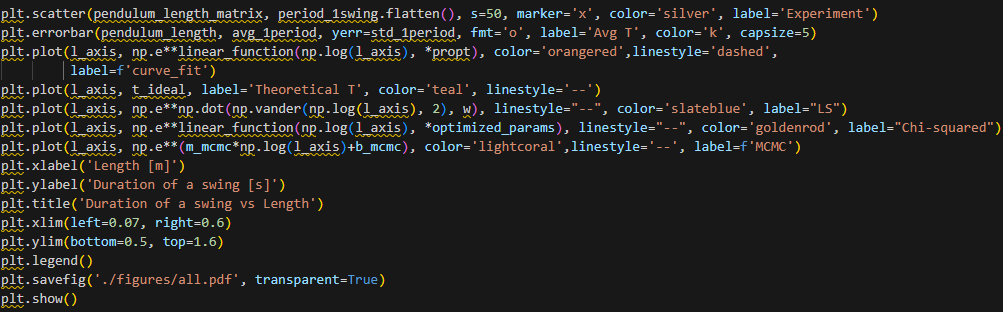
\includegraphics[width=1\linewidth]{CAM2.png}
    \caption{比較不同方法\-程式碼(2)}
    \label{fig:CAM2}
\end{figure}

\indent 此為三種方法的對數擬合結果比較;輸出結果見Fig.\ref{fig:CAM}右圖。

\clearpage

\begin{figure}[h]
    \centering
    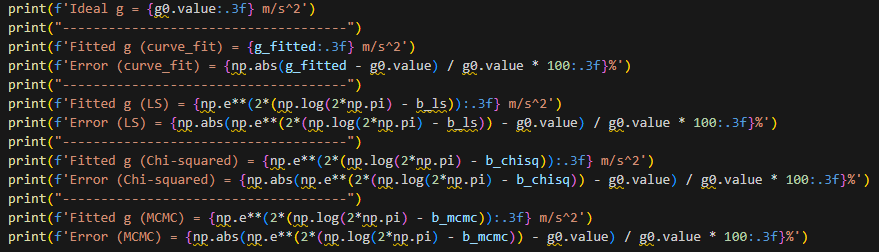
\includegraphics[width=1\linewidth]{CAM3.png}
    \caption{比較不同方法\-程式碼(3)}
    \label{fig:CAM3}
\end{figure}

\indent 此為三種方法推論出之重力加速度值。輸出得:\\
\begin{itemize}
    \item Ideal $g_0 = 9.807 \,m/s^2$
    \item $g_{(\texttt{curve\_fit})} = 9.807 \,m/s^2$\\$Error _{(\texttt{curve\_fit})} = 0.823\%$
    \item $g_{(LS)} = 9.969 \,m/s^2$\\$Error_{(LS)} = 1.660\%$
    \item $g_{(Chi-squared)} = 9.969 \,m/s^2$\\$Error _{(Chi-squared)} = 1.660\%$
    \item $g_{(MCMC)} = 9.887 \,m/s^2$\\$Error_{(MCMC)} = 0.823\%$
\end{itemize}

\begin{figure}[h]
    \centering    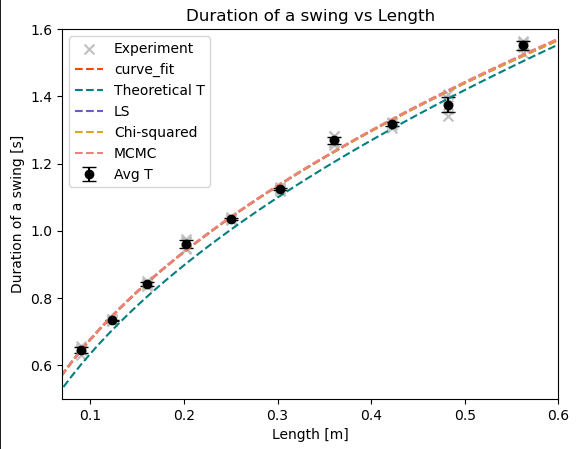
\includegraphics[width=0.45\linewidth]{CAMA.png} 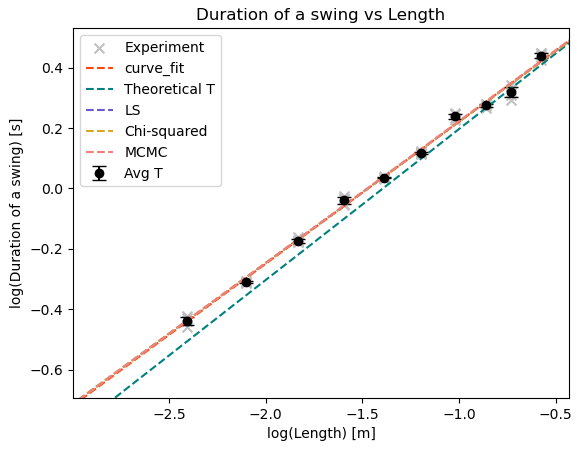
\includegraphics[width=0.45\linewidth]{CAMB.png}
    \caption{各方法比較之結果;左圖為線性擬合結果;右圖為對數擬合結果}
    \label{fig:CAM}
\end{figure}

\clearpage

\subsubsection{比較所有結果-數據分析}
\hfill

\indent 見Fig.\ref{fig:CAM},結果顯示各方法的擬合曲線接與平均值非常接近,尤其是\texttt{curve\_fit}和MCMC方法。右圖採用對數-對數圖表示資料和理論的線性關係,我們做出的圖顯示實驗資料大致服從$\log(T)\propto \frac{1}{2}\log(L) $的關係,理論模型有良好的預測性。\\
\indent 而因為我們在$\chi^2$ fitting雖有加權,但因為數據的標準差差異不大,因此在實作上幾乎等同於未加權最小平方法。

\subsubsection{比較所有結果-誤差討論}
\hfill

\indent 計算出之重力加速度誤差皆小於2\%,我們認為在可接受範圍內;LS和$\chi^2$值方法誤差較大,可能是因為在擬合過程中未考慮各資料點的不確定性(即週期的標準差),等於假設所有資料點的誤差相同,可能導致擬合結果對誤差較大的資料點過度信任,進而影響最終的斜率與g值;反之,\texttt{curve\_fit}與MCMC方法納入誤差加權機制,能更客觀反映實驗數據的實際變異性,因此其誤差相對較小。

\indent 改進方法:
\begin{enumerate}
    \item 誤差加權擬合:\\使用如 weighted least squares 或加權卡方分析,可更充分反映實驗誤差並提升擬合準確度。
    \item 增加測量次數:\\對每個擺長進行更多次的測量,有助於提升統計可靠度。
\end{enumerate}
\indent 實驗產生之系統誤差和隨機誤差,由於本次我們沒有實際做實驗,因而無法排除。


\clearpage
%%%%%%%%%%%%%%%%%%%%%%%%%%%%%%%%%%%%
\section{問題討論}

\subsection{根據實驗數據的擬合結果所計算出的$\chi^2$值是多少?如何利用$\chi^2$值判定擬合的好壞?如果值偏差較大,可能有哪些原因?}
\hfill
\begin{enumerate}
    \item 我們透過程式碼所計算出的$\chi^2$值為:0.15251356436613928
    \item 參考預習問題第四題及eq.(16),$\chi^2$表示的是測量值與預測值的加權平方差,誤差$\sigma_i$越小,偏差造成的影響越大;而應當透過自由度來分析使用$\chi^2$ fitting擬合的好壞。\\
    自由度定義為:衡量進行統計估計時有多少獨立的數據點或參數。\\
    數學表達:
    \begin{equation}
        \nu=N-p
    \end{equation}
    其中$\nu$為自由度;$N$為資料點之數量;$p$為擬合模型中參數的數量。
    比較每個自由度對應的$\chi^2$值:%因為 $\chi^2$ 值本身的大小受資料點數量和擬合參數數量的影響,因此直接比較原始 $\chi^2$ 值無法準確判斷擬合好壞
    \begin{equation}
        {\chi^2}_{reduced}=\frac{\chi^2}{\nu}=\frac{\chi^2}{N-p}
    \end{equation}
    這樣可以去除不同資料量或擬合參數量的影響,更直觀的表示出來
    \begin{itemize}
        \item 理想情況:\\在理想狀態下,每個自由度對應的卡方值會接近1,表示實驗值與觀察值間的差異和誤差範圍相應,無過多偏差。
        \item 過度擬合:\\若每個自由度對應的 $\chi^2$ 值顯著小於1,表示模型過度擬合資料,模型過於複雜,亦可能對資料的雜訊進行擬合,進而導致過度擬合的情況。
        \item 欠擬合:\\若每個自由度對應的 $\chi^2$ 值遠大於1,表示模型無法適配欲擬合之資料,可能原因為模型過於簡單,或數據的變化沒被捕捉到。
    \end{itemize}

    \item 若$\chi^2$值偏差較大,可能的原因如下:
    \begin{enumerate}
        \item 模型選擇不合適
        \item 誤差範圍估算錯誤
        \item 資料本身雜訊過多
    \end{enumerate}
        
\end{enumerate}

\subsection{在數據擬合過程中,測量誤差 (error bar) 的值會如何影響$\chi^2$值和最終擬合的重力加速度g?}
\hfill
\begin{enumerate}
    \item 同樣參考eq.(16),$\sigma_i$即表示數據的測量誤差,由此公式可見,$\sigma_i$會直接影響每個數據點對$\chi^2$的貢獻;當誤差較小(也就是$\sigma_i$較小)時,術據點之偏差($y_i - f(x_i)$)在$\chi^2$中的權重會變大;反之誤差變大時,此偏差將對$\chi^2$影響較小,導致整體的$\chi^2$更容易變小。

    \item 對最終擬合結果(重力加速度g)的影響:
    \begin{itemize}
        \item 當誤差較小時,數據點的偏差會在擬合過程會得到更大影響,模型將更顯著的調整參數,以減少誤差;使得最終擬合結果更為精確。
        \item 當誤差較大時,數據點的偏差對擬合的影響較小,擬合過程會更仰賴於較大的誤差範圍,使最終擬合結果可能產生較大的不確定性。
    \end{itemize}
\end{enumerate}
%%%%%%%%%%%%%%%%%%%%%%%%%%%%%%%%%%%%%
\subsection{殘差圖是否呈現隨機分佈?是否觀察到某種趨勢(例如隨擺長增加或減少)?如果存在系統性誤差,可能的原因是什麼?如何改進實驗設計來減少這類誤差?}
\hfill

\indent 根據殘差圖Fig.\ref{fig:chiB}顯示,殘差接分布於殘差值$=0$之附近,因此無法從殘差圖中觀察並推斷出殘差具有任何趨勢關係。因此我們可以暫時推論殘差屬於機率分布,與擺長並沒有關聯。若要驗證推論,則可以透過實際實驗取得數據,確認不同擺長下的殘差圖是否依舊符合隨機分布。\\
\indent 系統性誤差可能來源:
\begin{enumerate}
    \item 單擺擺動時可能受到空氣阻力影響。\\解決方式:在真空環境下實驗。
    \item 量測誤差。\\解決方式:使用精確度更高的量測工具,包含更準確的計時器、量角器等等,或是透過機器、電腦操作計時和調整單擺擺放角度,避免人為操作產生之誤差。
\end{enumerate}


\subsection{$\chi^2$擬合的結果與單純使用最小二乘法(least square fitting)擬合相比有何不同?$\chi^2$擬合的優勢在哪裡?適合用在什麼實驗?}
\hfill

最小二乘法 (least square fitting)的核心概念是找出一條線,使得數據點與這條線垂直距離的平方和能達到最小值,即是殘差平方總和的最小化。

最小二乘法假設:
誤差是隨機分布、正態分布,並且每個點的誤差大小皆一樣大(稱為等變異性)、資料點之間相互獨立。最小二乘法較明顯的問題是其對異常值較敏感,因此若是數據之誤差值較大,其擬合結果可能偏差。

而$\chi^2$擬合則會考慮到測量誤差,如果數據點內的量測誤差大小不同,使用$\chi^2$擬合可確保誤差較大之數值不會對整體數據造成太明顯的影響。$\chi^2$值大表示觀察到的結果與期望值有較大差異,不確定度的較大數據之殘差會降低對$\chi^2$值的貢獻,反之不確定不小的數據之殘差則會提高對$\chi^2$值的貢獻。若測量誤差相同,$\chi^2$擬合結果會等於最小二乘法。

同時$\chi^2$擬合可以透過檢測P值確認擬合的可信度。故$\chi^2$擬合適用於誤差來源較多的實驗,如單擺實驗或者光譜實驗,透過使用$\chi^2$擬合,可以較有效地降低誤差帶來的干擾。



\section{總結}
\hfill

本實驗以驗證單擺週期與擺長之經典關係為目標,並利用 Chi-square 擬合方法分析實驗數據,進而反推出重力加速度值。Chi-square 擬合的一大優點為其可根據資料的誤差給予不同權重,使誤差較小的資料點對模型更具影響力。在本次實作中,我們透過最小化卡方統計量,求得擬合參數$m=0.4802$、$b=0.7927$,計算得$g=9.969 \,m/s^2$,與理論值$g=9.807 \,m/s^2$相比誤差為 1.66\%。然而,$\chi^2=0.1525$ 遠小於自由度(8),顯示模型或誤差估計可能存在過度樂觀的情形。從殘差圖觀察,資料點大致隨機分佈,無明顯系統性誤差,顯示擬合結果具統計合理性。此外,我們亦將Chi-square 擬合與其他方法(如最小平方法、\texttt{curve\_fit}與MCMC)進行比較,發現考慮誤差加權的擬合方法(如 \texttt{curve\_fit} 與MCMC)在精確度與穩定性上表現更佳,凸顯了誤差估計與模型選擇在實驗分析中的重要性。

\clearpage

\section{分工}

洪懌平:coding、前言\\
黃巧涵:\texttt{curve\_fit}、LS數據分析及誤差討論、問題三四\\
洪瑜:$\chi^2$ fitting、MCMC數據分析及誤差討論、問題一二


%--------------------------------------------------------------
\end{CJK}
\end{document}